%\VignetteIndexEntry{The qsmooth user's guide}
%\VignettePackage{qsmooth}
%\VignetteEngine{knitr::knitr}
\documentclass{article}

\RequirePackage[]{/Library/Frameworks/R.framework/Versions/3.3/Resources/library/BiocStyle/resources/tex/Bioconductor2}
\AtBeginDocument{\bibliographystyle{/Library/Frameworks/R.framework/Versions/3.3/Resources/library/BiocStyle/resources/tex/unsrturl}}
\usepackage[noae, nogin]{Sweave}
\setlength{\parskip}{1\baselineskip}
\setlength{\parindent}{0pt}

\title{The \texttt{qsmooth} user's guide}
\author[1,2]{Stephanie C. Hicks}
\author[3]{Kwame Okrah}
\author[1,2]{Joseph Paulson}
\author[1,2]{John Quackenbush}
\author[1,2]{Rafael A. Irizarry}
\author[4,5]{Hector Corrada Bravo}
\affil[1]{Department of Biostatistics and Computational Biology, Dana-Farber Cancer Institute}
\affil[2]{Department of Biostatistics, Harvard T.H. Chan School of Public Health}
\affil[3]{Genentech}
\affil[4]{Department of Computer Science, University of Maryland, College Park}
\affil[5]{Center for Bioinformatics and Computational Biology, Institute of Advanced Computer Studies, University of Maryland, College Park}


\date{Modified: February 15, 2017.  Compiled: \today}

\usepackage{Sweave}
\begin{document}
\Sconcordance{concordance:qsmooth-vignette.tex:qsmooth-vignette.Rnw:%
1 5 1 49 0 3 1 1 0 117 1 4 0 19 1 4 0 20 1 17 0 15 1 17 0 76 1 6 0 8 1 6 0 53 1 %
6 0 11 1 6 0 20 1 47 0 4 1}



\maketitle

\tableofcontents

\section{Introduction}

Global normalization methods such as quantile normalization
\cite{Bolstad2003, Irizarry2003} have become a standard part of the
analysis pipeline for high-throughput data to remove unwanted
technical variation. These methods and others that rely solely
on observed data without external information (e.g. spike-ins)
are based on the assumption that only a minority of genes are
expected to be differentially expressed (or that an equivalent
number of genes increase and decrease across biological conditions
\cite{aanes2014normalization}). This assumption can be interepreted
in different ways leading to different global normalization
procedures. For example, in one normalization procedure, the method assumes
the mean expression level across genes should be the same across samples
\cite{Robinson2010}. In contrast, quantile normalization assumes the
only difference between the statistical distribution of each sample
is technical variation. Normalization is achieved by forcing the
observed distributions to be the same and the average distribution,
obtained by taking the average of each quantile across samples,
is used as the reference \cite{Bolstad2003}.

While these assumptions may be reasonable in certain experiments,
they may not always be appropriate \cite{Loven2012, Hicks2015}.
For example, mRNA content has been shown to fluctuate significantly
during zebrafish early developmental stages \cite{aanes2014normalization}.
Similarily, cells expressing high levels of c-Myc undergo
transcriptional amplification causing a 2 to 3 fold change in global
gene expression compared to cells expressiong low c-Myc
\cite{Loven2012}.

Recently, an R/Biocoductor package (\texttt{quantro}) \cite{Hicks2015}
has been developed to test for global differences between groups of
distributions to evaluate whether global normalization methods such
as quantile normalization should be applied. If global differences
are found between groups of distributions, these changes may be of technical
or biological of interest. If these changes are of technical interest
(e.g. batch effects), then global normalization methods should be applied.
If these changes are related to a biological covariate (e.g. normal/tumor or
two tissues), then global normalization methods should not be applied
because the methods will remove the interesting biological variation
(i.e. differentially expressed genes) and artifically induce differences
between genes that were not differentially expressed. In the cases
with global differences between groups of distributions
between biological conditions, quantile normalization is
not an appropriate normalization method. In
these cases, we can consider a more relaxed assumption about the data,
namely that the statistical distribution of each sample should be the
same within biological conditions or groups (compared to the more
stringent assumption of quantile normalization, which states the
statistical distribution is the same across all samples).

In this vignette we introduce a generalization of quantile
normalization, referred to as \textbf{smooth quantile normalization}
(\textbf{qsmooth}), which is a weighted average of the two
types of assumptions about the data. The \texttt{qsmooth} R-package
contains the \texttt{qsmooth()} function, which computes a weight at
every quantile that compares the variability between groups relative
to within groups. In one extreme, quantile normalization is applied
and in the other extreme quantile normalization within each
biological condition is applied. The weight shrinks the group-level
quantile normalized data towards the overall reference quantiles
if variability between groups is sufficiently smaller than the
variability within groups. The algorithm is described in
Figure \ref{algo} below.

Let \texttt{gene(g)} denote the ${g}^{th}$ row after sorting
each column in the data. For each row, \texttt{gene(g)}, we
compute the weight $w_{(g)} \in [0, 1]$, where a weight of 0 implies
quantile normalization within groups is applied and
a weight of 1 indicates quantile normalization is applied.
The weight at each row depends on the between group sum of squares
$\hbox{SSB}_{(g)}$ and total sum of squares $\hbox{SST}_{(g)}$,
as follows:
\begin{equation}
w_{(g)} = \hbox{median} \{1 - \hbox{SSB}_{(i)} / \hbox{SST}_{(i)} | ~i = g-k, \dots, g, \dots, g+k \},
\end{equation}
where $k=$ floor(Total number of genes * 0.05). The number
0.05 is a flexible parameter that can be altered to change the
window of the number of genes considered. In this way, we
can use a rolling median to borrow information from
neighboring genes in the weight.

\begin{figure}[!h]
\begin{center}
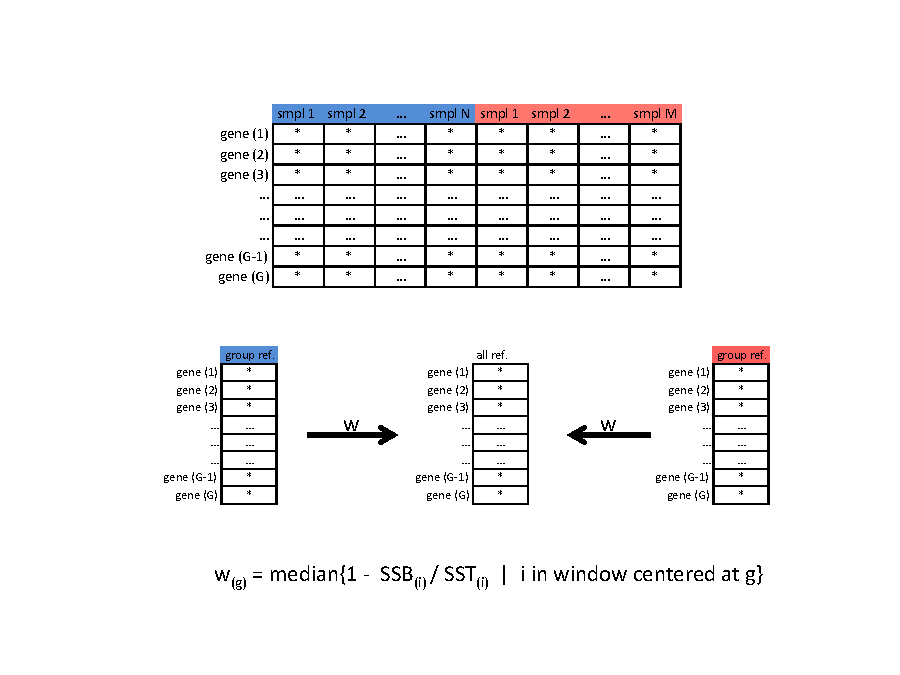
\includegraphics[width=\columnwidth]{qsmooth_algo.pdf}
\end{center}
\small\normalsize
\caption[qsmooth algorithm]
         {{\bf The qsmooth algorithm}}
\label{algo}
\end{figure}


\section{Getting Started}

Load the package in R
\begin{Schunk}
\begin{Sinput}
> library(qsmooth)
\end{Sinput}
\end{Schunk}


\section{Data}

The \textbf{bodymapRat} package contains an
\texttt{ExpressionSet} of 652 RNA-Seq samples from a comprehensive
rat transcriptomic BodyMap study. This data was derived from
the raw FASTQ files obtained from Yu et al. (2014) \cite{Yu2014}.
It contains expression levels from 11 organs in male and female
rats at 4 developmental stages. We will use a subset of this
data in this vignette.

The R-package bodymapRat can be installed from GitHub using the R package
\textbf{devtools}.

\begin{Schunk}
\begin{Sinput}
> library(devtools)
> install_github("stephaniehicks/bodymapRat")
\end{Sinput}
\end{Schunk}


\subsection{bodymapRat Example 1 - Comparing male and female rats in one tissue}

The first example is based a dataset
which contains lung samples from 21 week old male and female rats.
Four samples are from males and four samples are from females.

\begin{Schunk}
\begin{Sinput}
> library(Biobase)
> library(bodymapRat)
> data(bodymapRat)
> # select lung samples, stage 21 weeks, and only bio reps
> keepColumns = (pData(bodymapRat)$organ == "Lung") &
+     (pData(bodymapRat)$stage == 21) & (pData(bodymapRat)$techRep == 1)
> keepRows = rowMeans(exprs(bodymapRat)) > 10 # Filter out low counts
> bodymapRatE1 <- bodymapRat[keepRows,keepColumns]
> bodymapRatE1
\end{Sinput}
\begin{Soutput}
ExpressionSet (storageMode: lockedEnvironment)
assayData: 18629 features, 8 samples 
  element names: exprs 
protocolData: none
phenoData
  sampleNames: SRR1170173 SRR1170175 ... SRR1170213 (8 total)
  varLabels: sraExperiment sraRun ... ytile (22 total)
  varMetadata: labelDescription
featureData: none
experimentData: use 'experimentData(object)'
Annotation:  
\end{Soutput}
\end{Schunk}

\subsection{bodymapRat Example 2 - Comparing two tissues}

The second example is based a dataset which contains brain and liver
tissue samples from 21 week old male and female rats.
eight samples are from males and eight samples are from females.

\begin{Schunk}
\begin{Sinput}
> # select brain and liver samples, stage 21 weeks, and only bio reps
> keepColumns = (pData(bodymapRat)$organ %in% c("Brain", "Liver")) &
+          (pData(bodymapRat)$stage == 21) & (pData(bodymapRat)$techRep == 1)
> keepRows = rowMeans(exprs(bodymapRat)) > 10 # Filter out low counts
> bodymapRatE2 <- bodymapRat[keepRows,keepColumns]
> bodymapRatE2
\end{Sinput}
\begin{Soutput}
ExpressionSet (storageMode: lockedEnvironment)
assayData: 18629 features, 16 samples 
  element names: exprs 
protocolData: none
phenoData
  sampleNames: SRR1169975 SRR1169977 ... SRR1170277 (16 total)
  varLabels: sraExperiment sraRun ... ytile (22 total)
  varMetadata: labelDescription
featureData: none
experimentData: use 'experimentData(object)'
Annotation:  
\end{Soutput}
\end{Schunk}

\section{Using the \texttt{qsmooth() function}}


\subsection{Input for \texttt{qsmooth()}}
The \texttt{qsmooth()} function must have two objects as input:

\begin{itemize}
\item \texttt{object}: a data frame or matrix with observations
(e.g. probes or genes) on the rows and samples as the columns.
\texttt{qsmooth()} can accept objects that inherit \texttt{eSets}
such as an \texttt{ExpressionSet} or \texttt{MethylSet}. In this case,
the \texttt{groupFactor} must still be provided.
\item \texttt{groupFactor}: a continuous or categorial covariate
that represents the group level biological variation about each sample.
For example if the samples represent two different tissues,
provide \texttt{qsmooth()} with a covariate representing
which columns in the \texttt{object} are different tissue samples.
\item \texttt{batch}: {\bf optional} batch covariate (multiple
batches are not allowed). If batch covariate is provided,
\texttt{ComBat()} from \texttt{sva} is used prior to
qsmooth normalization to remove batch effects.
See \texttt{ComBat()} for more details.
\item \texttt{normFactors}: {\bf optional} scaling normalization factors.
Default is \texttt{NULL}. If \texttt{normFactors} is not equal to
\texttt{NULL}, the user can provide a vector of scaling factors
that will be used to modify the expression data set prior to
applying the \texttt{qsmooth} algorithm.
\item \texttt{window}: window size for running median (defined as a
fraction of the number of rows of exprs. Default is 0.05
\end{itemize}



\subsection{Running \texttt{qsmooth()}}

\subsubsection{Using Example 1 data}
In the first example, the groups we are interested in comparing are
contained in the \texttt{sex} column in the \texttt{pData(bodymapRatE1)}
dataset. To run the \texttt{qsmooth()} function, input the data object
and the object containing the phenotypic data. Here we use the
\texttt{bodymapRatE1} data set as an example.

The first row shows the boxplots and density plot of the raw data that
has been transformed on the \texttt{log2()} scale and added a
pseudo-count of 1 (i.e. \texttt{log2(counts+1)}).

The second row shows the boxplots and density plot of the qsmooth
normalized data.


\begin{Schunk}
\begin{Sinput}
> library(quantro)
> par(mfrow=c(2,2))
> pd1 <- pData(bodymapRatE1)
> eset1_ercc <- exprs(bodymapRatE1)[grepl("^ERCC", rownames( exprs(bodymapRatE1))), ]
> eset1 <- exprs(bodymapRatE1)[!grepl("^ERCC", rownames( exprs(bodymapRatE1))), ]
> matboxplot(log2(eset1+1), groupFactor = pd1$sex, main = "Raw data",
+            ylab = "Expression (log2 scale)", xaxt="n")
> axis(1, at=seq_len(length(pd1$sex)), labels=FALSE)
> text(seq_len(length(pd1$sex)), par("usr")[3] -1, labels = pd1$sex, srt = 90, pos = 1, xpd = TRUE)
> matdensity(log2(eset1+1), groupFactor = pd1$sex, main = "Raw data",
+            xlab = "Expression (log2 scale)", ylab = "density")
> legend('topright', levels(factor(pd1$sex)), col = 1:2, lty = 1)
> qsNormE1 <- qsmooth(object = eset1, groupFactor = pd1$sex)
> matboxplot(log2(qsmoothData(qsNormE1)+1), groupFactor = pd1$sex,
+            main = "qsmooth normalized data", ylab = "Expression (log2 scale)",
+            xaxt="n")
> axis(1, at=seq_len(length(pd1$sex)), labels=FALSE)
> text(seq_len(length(pd1$sex)), par("usr")[3] -1, labels = pd1$sex, srt = 90, pos = 1, xpd = TRUE)
> matdensity(log2(qsmoothData(qsNormE1)+1), groupFactor = pd1$sex,
+            main = "qsmooth normalized data",
+            xlab = "Expression (log2 scale)", ylab = "density")
> legend('topright', levels(factor(pd1$sex)), col = 1:2, lty = 1)
\end{Sinput}
\end{Schunk}
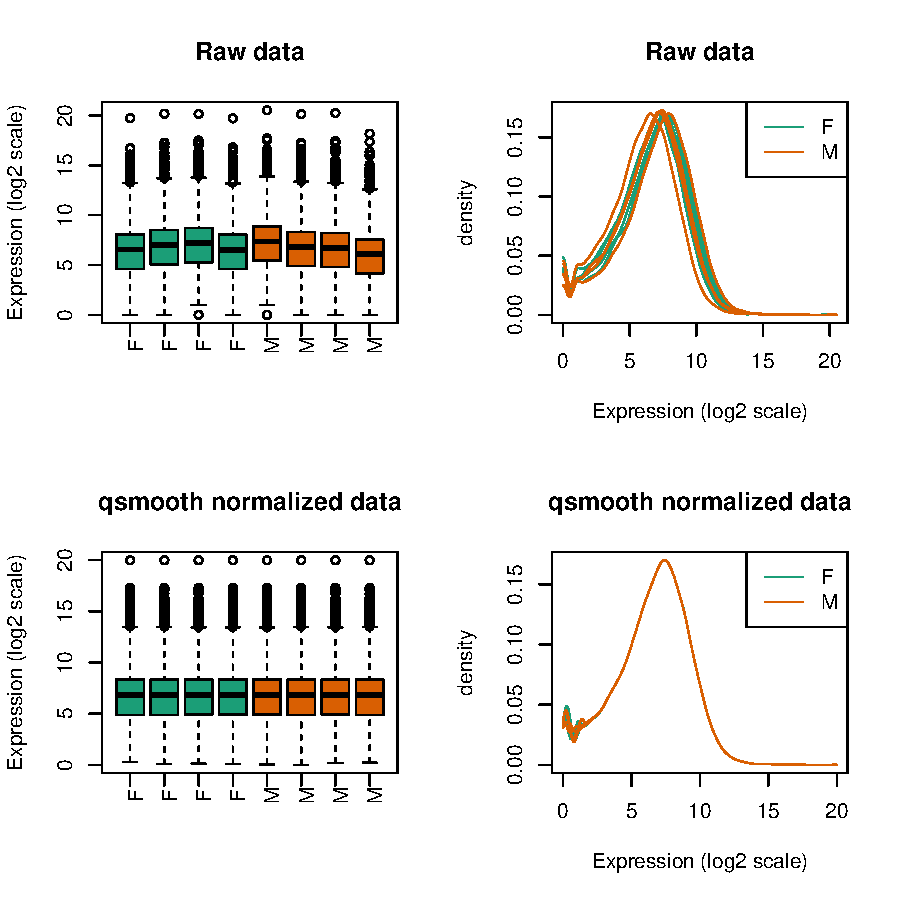
\includegraphics{qsmooth-vignette-calculate-qsmooth1}


The smoothed quantile normalized data can be extracted using the
\texttt{qsmoothData()} function (see above) and the smoothed quantile weights
can plotted using the \texttt{qsmoothPlotWeights()} function (see below).

\begin{Schunk}
\begin{Sinput}
> qsmoothPlotWeights(qsNormE1)
\end{Sinput}
\end{Schunk}
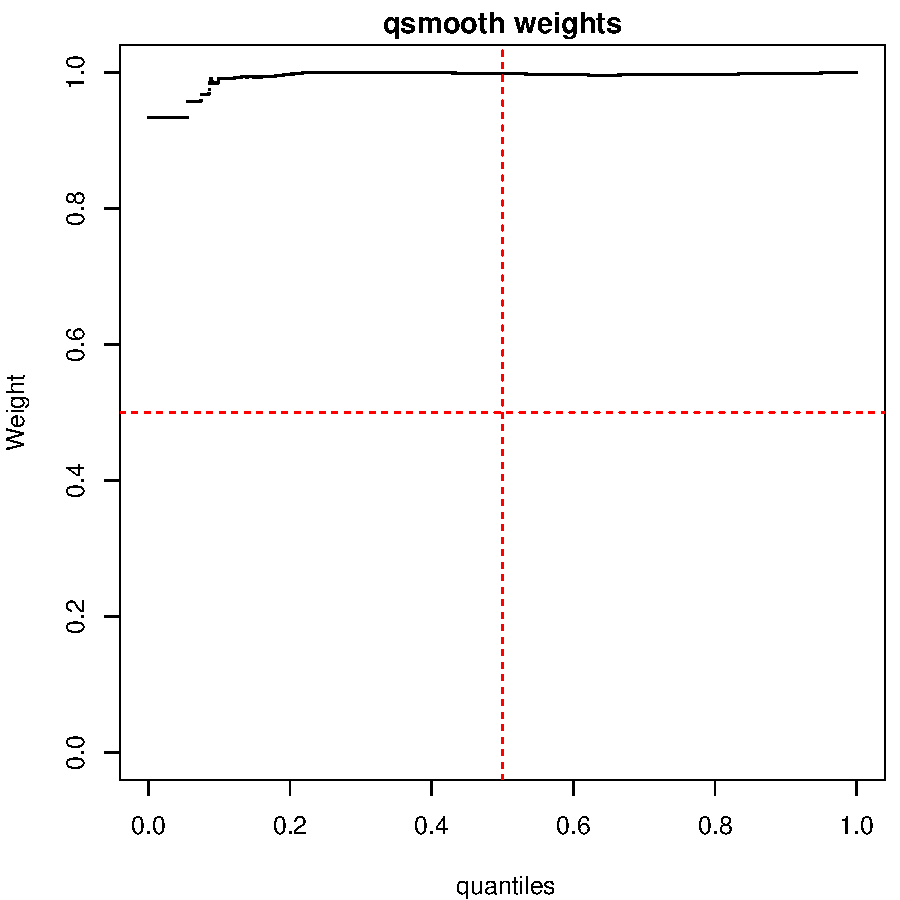
\includegraphics{qsmooth-vignette-plot-qsmooth1-weights}


The weights are calculated for each quantile in the data set.
A weight of 1 indicates quantile normalization is applied,
where as a weight of 0 indicates quantile normalization
within the groups is applied. See Figure \ref{algo} for
more details on the weights.

In this example, the weights are close to 1 across all the
quantiles indicating that there is no major difference
between the group-level quantiles in the female and male rats.
Here, the \texttt{qsmooth()} normalization method returns a
normalized data set that is nearly identical
to the conventional quantile normalization.


\subsubsection{Using Example 2 data}

In the second example (\texttt{bodymapRatE2}), the groups we
are interested in comparing are the two types of tissues in
the 21 week old male and female rats.

Similar to the first example, the first row shows the boxplots
and density plot of the raw data that has been transformed on
the \texttt{log2()} scale and added a pseudo-count of 1
(i.e. \texttt{log2(counts+1)}). The second row shows the boxplots
and density plot of the qsmooth normalized data.

\begin{Schunk}
\begin{Sinput}
> par(mfrow=c(2,2))
> pd2 <- pData(bodymapRatE2)
> eset2_ercc <- exprs(bodymapRatE2)[grepl("^ERCC", rownames( exprs(bodymapRatE2))), ]
> eset2 <- exprs(bodymapRatE2)[!grepl("^ERCC", rownames( exprs(bodymapRatE2))), ]
> pd2$group <- paste(pd2$organ, pd2$sex, sep="_")
> matboxplot(log2(eset2+1), groupFactor = factor(pd2$organ), main = "Raw data",
+            ylab = "Expression (log2 scale)", xaxt="n")
> axis(1, at=seq_len(length(as.character(pd2$organ))), labels=FALSE)
> text(seq_len(length(pd2$organ)), par("usr")[3] -2, labels = pd2$organ, srt = 90, pos = 1, xpd = TRUE)
> matdensity(log2(eset2+1), groupFactor = pd2$organ, main = "Raw data",
+            xlab = "Expression (log2 scale)", ylab= "density")
> legend('topright', levels(factor(pd2$organ)), col = 1:2, lty = 1)
> qsNormE2 <- qsmooth(object = eset2, groupFactor = pd2$organ)
> matboxplot(log2(qsmoothData(qsNormE2)+1), groupFactor = pd2$organ,
+            main = "qsmooth normalized data", ylab = "Expression (log2 scale)",
+            xaxt="n")
> axis(1, at=seq_len(length(pd2$organ)), labels=FALSE)
> text(seq_len(length(pd2$organ)), par("usr")[3] -2, labels = pd2$organ, srt = 90, pos = 1, xpd = TRUE)
> matdensity(log2(qsmoothData(qsNormE2)+1), groupFactor = pd2$organ,
+            main = "qsmooth normalized data",
+            xlab = "Expression (log2 scale)", ylab = "density")
> legend('topright', levels(factor(pd2$organ)), col = 1:2, lty = 1)
\end{Sinput}
\end{Schunk}
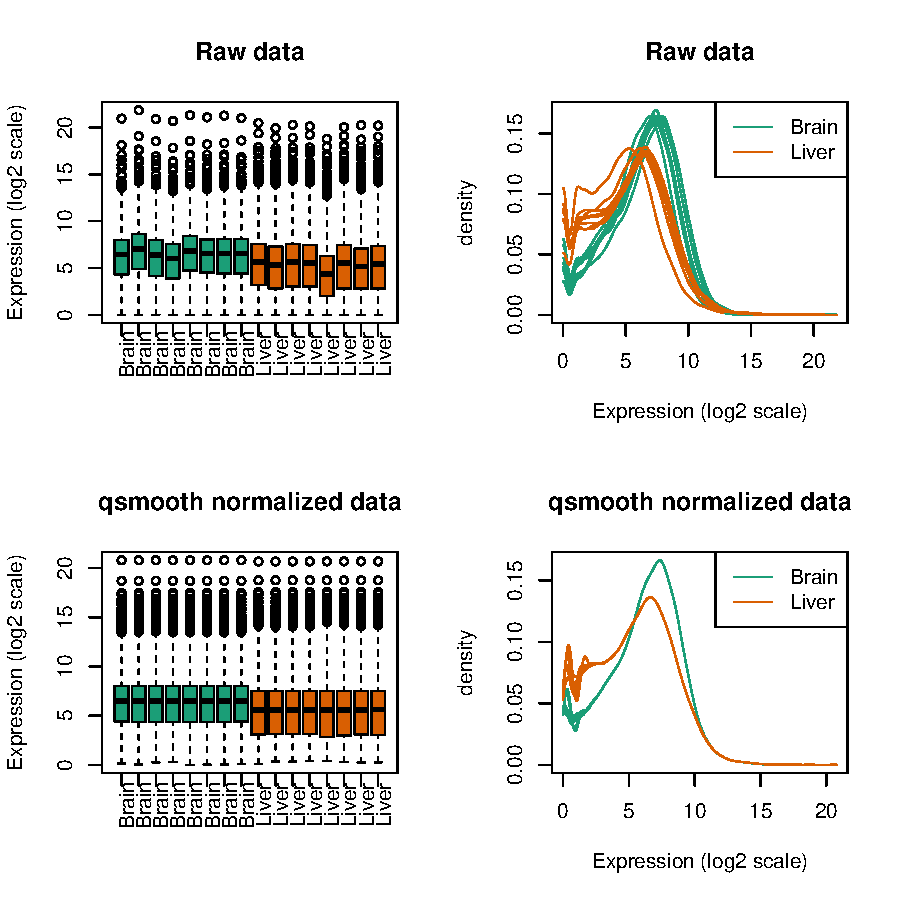
\includegraphics{qsmooth-vignette-calculate-qsmooth2}

We see there are global differences in the distributions between the
two tissues (liver and brain) in the rats.

The smoothed quantile normalized data can be extracted using the
\texttt{qsmoothData()} function (see above) and the smoothed quantile weights
can plotted using the \texttt{qsmoothPlotWeights()} function (see below).

\begin{Schunk}
\begin{Sinput}
> qsmoothPlotWeights(qsNormE2)
\end{Sinput}
\end{Schunk}
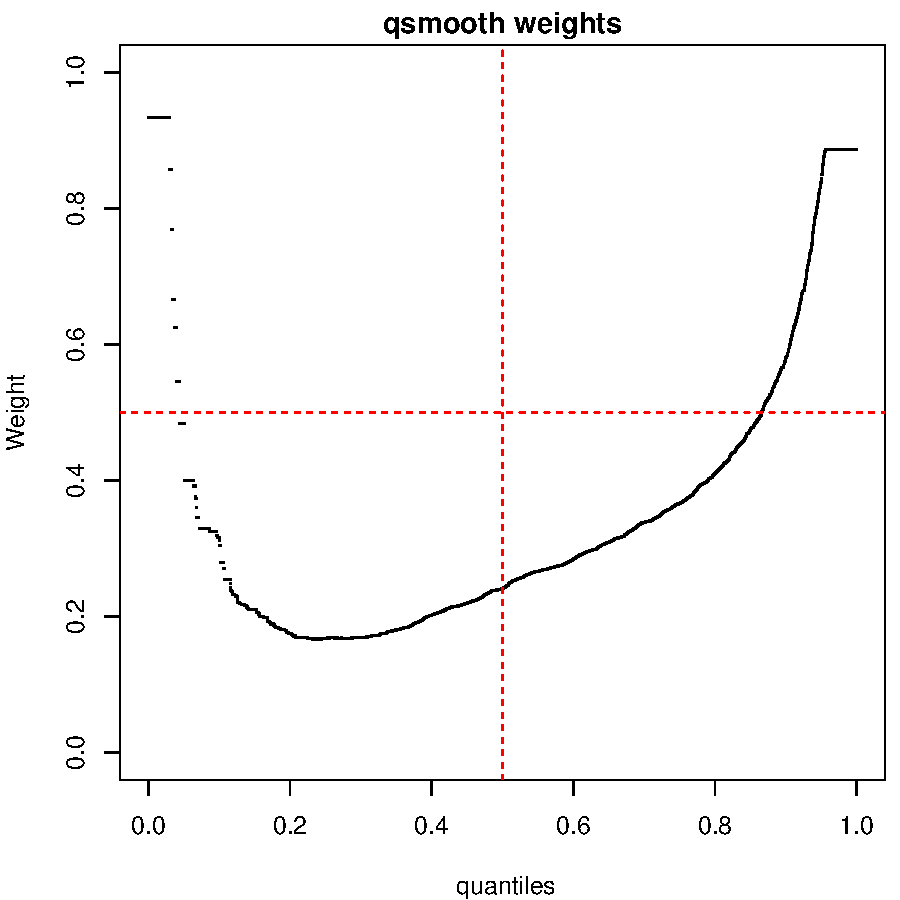
\includegraphics{qsmooth-vignette-plot-qsmooth2-weights}

Recall, a weight of 1 indicates quantile normalization is applied,
where as a weight of 0 indicates quantile normalization
within the groups is applied.

In this example, the weights range from 0.2 to 0.8 across the quantiles,
where the weights are close to 0.2 for the quantiles close to 0 and the
weights are close to 0.8 for the quantiles close to 1.
This plot suggests the distributions contain more variablity between
the groups compared to within groups for the small quantiles (and
the conventional quantile normalization is not necessarily appropriate).
As the quantiles get bigger, there is less variability between groups which
increases the weight closer to 0.8 as the quantiles get bigger.


\section{SessionInfo}

\begin{Schunk}
\begin{Sinput}
> sessionInfo()
\end{Sinput}
\begin{Soutput}
R version 3.3.2 (2016-10-31)
Platform: x86_64-apple-darwin13.4.0 (64-bit)
Running under: OS X El Capitan 10.11.6

locale:
[1] en_US.UTF-8/en_US.UTF-8/en_US.UTF-8/C/en_US.UTF-8/en_US.UTF-8

attached base packages:
[1] parallel  stats     graphics  grDevices datasets  utils    
[7] methods   base     

other attached packages:
[1] quantro_1.6.2       bodymapRat_0.0.1    Biobase_2.32.0     
[4] BiocGenerics_0.18.0 qsmooth_0.0.1      

loaded via a namespace (and not attached):
 [1] mclust_5.2                 base64_2.0                
 [3] Rcpp_0.12.7                locfit_1.5-9.1            
 [5] lattice_0.20-34            Rsamtools_1.24.0          
 [7] Biostrings_2.40.2          digest_0.6.10             
 [9] foreach_1.4.3              R6_2.1.3                  
[11] GenomeInfoDb_1.8.7         plyr_1.8.4                
[13] chron_2.3-47               stats4_3.3.2              
[15] RSQLite_1.0.0              httr_1.2.1                
[17] bumphunter_1.12.0          ggplot2_2.1.0             
[19] zlibbioc_1.18.0            GenomicFeatures_1.24.5    
[21] data.table_1.9.6           annotate_1.50.0           
[23] S4Vectors_0.10.3           Matrix_1.2-7.1            
[25] preprocessCore_1.34.0      splines_3.3.2             
[27] BiocParallel_1.6.6         stringr_1.1.0             
[29] munsell_0.4.3              RCurl_1.95-4.8            
[31] biomaRt_2.28.0             rtracklayer_1.32.2        
[33] multtest_2.28.0            pkgmaker_0.22             
[35] openssl_0.9.4              SummarizedExperiment_1.2.3
[37] GEOquery_2.38.4            quadprog_1.5-5            
[39] IRanges_2.6.1              codetools_0.2-15          
[41] matrixStats_0.50.2         XML_3.98-1.4              
[43] reshape_0.8.5              GenomicAlignments_1.8.4   
[45] MASS_7.3-45                bitops_1.0-6              
[47] grid_3.3.2                 nlme_3.1-128              
[49] xtable_1.8-2               gtable_0.2.0              
[51] registry_0.3               DBI_0.5-1                 
[53] magrittr_1.5               scales_0.4.0              
[55] stringi_1.1.1              XVector_0.12.1            
[57] genefilter_1.54.2          doRNG_1.6                 
[59] doParallel_1.0.10          limma_3.28.21             
[61] minfi_1.18.6               nor1mix_1.2-2             
[63] BiocStyle_2.0.3            RColorBrewer_1.1-2        
[65] iterators_1.0.8            siggenes_1.46.0           
[67] tools_3.3.2                illuminaio_0.14.0         
[69] rngtools_1.2.4             survival_2.39-5           
[71] colorspace_1.2-6           AnnotationDbi_1.34.4      
[73] GenomicRanges_1.24.3       beanplot_1.2              
\end{Soutput}
\end{Schunk}

\bibliography{qsmoothRef}

\end{document}
